\section{\hologo{TeX}\,Live}
\label{sec:tl}

\hologo{TeX}\,Live 是目前使用最为广泛的 \hologo{TeX} 发行版,支持 Windows、Linux 和 macOS。其中,在 macOS 上发行的版本称为 Mac\hologo{TeX}。
这个发行版的特点是\emph{大而全}:多数情况下,你会使用 \texttt{full-scheme} 安装 多达 7 GB 的完整发行版\sidenote{这当然是因为 tlmgr 不会像 pip 一样智能管理依赖项。比方说我也许一辈子都用不到其中跟挪威语有关的宏包,真是气抖冷。},而这另一方面也带来了可以说最正统的 \TeX{} 体验。

\subsection{前提条件}

一台正常访问校园网的设备,详见 \ref{subsec:device}。

\subsection{或许有些不合时宜……}

\hologo{TeX}\,Live 以年份为版本号,在每年 4 月 1 日左右发布新版本,一般不能无缝进行版本升级\sidenote{只能卸载旧版、从头安装新版。旧版本的 tlmgr 无法拉取到宏包更新。}。当前(2022年3月)正处于 \hologo{TeX}\,Live 2022 的发布前夕\sidenote{Plan for TeX Live 2022:\\
\tiny
22mar: final updates from CTAN, final doc tweaks.\\
3apr: public release (also of MacTeX).},建议再考虑考虑。

如果你后悔了,还可以到第一页重新选择。

如果你执意前行,这里是空降链接:
\hyperref[subsec:tl-win]{\faWindows{}}\,
\hyperref[subsec:tl-linux]{\faLinux{}}\,
\hyperref[subsec:tl-mac]{\faApple{}}

\subsection{Windows}
\label{subsec:tl-win}

\begin{widepar}
可能是出于文件 IO 效率原因,\TeX{} 排版系统在 Windows 系统下的表现并不优秀,不仅体现在编译速度稍慢于 UNIX,也在于过长的安装时间。以下首要推荐\emph{镜像安装方法};如果你对自己的电脑性能和网络连接质量很有信心,也可以试试在线安装。
\end{widepar}

\subsubsection{镜像安装}
\label{subsubsec:tl-from-iso}

\begin{widepar}
每年更新版本时会发布一个巨大无比的安装镜像,点击链接获取:
\end{widepar}

\begin{itemize}
  \item \href{https://mirrors.nju.edu.cn/CTAN/systems/texlive/Images/texlive2021-20210325.iso}{\faFile*[regular] \texttt{texlive2021-20210325.iso}}
\end{itemize}

双击打开下载的 ISO 文件,Windows 会自动挂载到虚拟光驱\sidenote{也有可能 \texttt{.iso} 文件被当作压缩文件,这就要将其完整解压缩到一个路径不含中文的文件夹下面。},弹出一个新的文件夹窗口。接着,需要在右键菜单中\emph{以管理员身份运行} \texttt{install-tl-windows.bat},稍等片刻,会呈现如图~\ref{fig:install-tl-0} 所示的窗口。

\begin{figure}[htbp]
  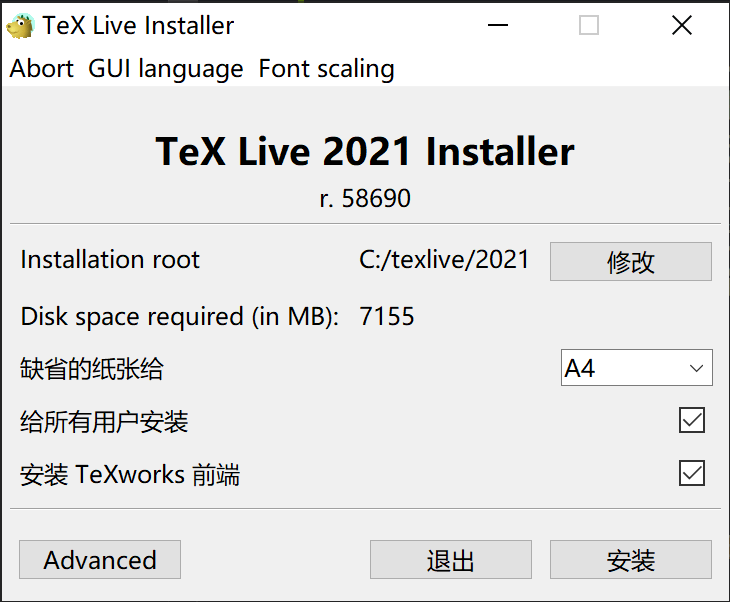
\includegraphics[width=0.45\textwidth]{install-tl-0}
  \caption{安装器,版本 \texttt{r. 58690}。}
  \label{fig:install-tl-0}
\end{figure}

保持默认设置\sidenote{也可以选择不装 TeXworks 编辑器},点击“安装”按钮。安装将耗费至少 20 分钟时间,在某些型号的电脑上甚至可能超过一个小时\sidenote{什么,刚开始就报错?再看看前提条件的用户文件夹名称问题吧!}。出门吃个饭吧!

全部完成后可以关闭安装程序,接着阅读 \ref{sec:hw}。

但如果你仍然闲着,可以把宏包都更新一遍,毕竟是去年 3 月份打包的。以管理员身份打开终端\sidenote{忘了怎么做?回去看看 \ref{subsec:terminal}。},执行下面的命令:

\vspace*{-0.7cm}
\begin{widepar}
\begin{shellexample}[morekeywords={tlmgr,fmtutil-user},emph={option,update},
  xleftmargin = 0.5 em, xrightmargin = 1 em]
  tlmgr option repository https://mirrors.nju.edu.cn/CTAN/systems/texlive/tlnet
  tlmgr update --self --all
  fmtutil-user --all
\end{shellexample}
\end{widepar}

升级操作也会持续挺久。再找点别的事情做吧。

\subsubsection{在线安装}
\label{subsubsec:tl-from-net}

\begin{widepar}
在线安装的优势在于所有宏包装上就是最新版。只需下载一个小巧的安装器:
\end{widepar}

\begin{itemize}
  \item \href{https://mirrors.nju.edu.cn/CTAN/systems/texlive/tlnet/install-tl.zip}{\faFile*[regular] \texttt{install-tl.zip}}
\end{itemize}

完整解压缩到一个路径不含中文的文件夹下面,在右键菜单中\emph{以管理员身份运行} \texttt{install-tl-windows.bat},就会弹出安装器窗口。这时赶紧用 “Specify mirror...” 找到我们学校的镜像!\sidenote{位于 Asia -> China -> https://mirrors.nju.edu.cn/...,其实不指定南大源也没问题,但据说校内用起来确实快一点。}

\begin{figure}[htbp]
  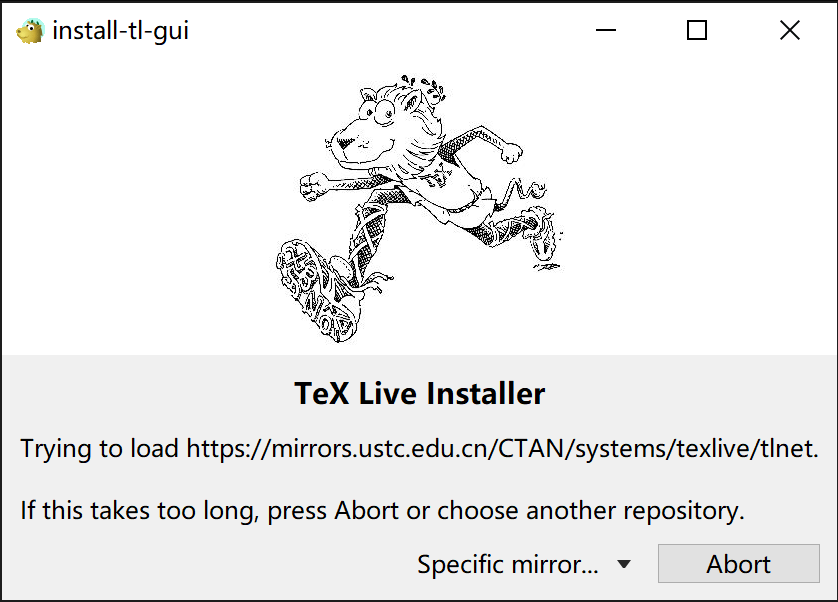
\includegraphics[width=0.45\textwidth]{install-tl-1}
  \caption{在线安装第一步。一定要动作快,不然镜像源就自动设置到隔壁中科大了!}
\end{figure}

\begin{widepar}
接下来的步骤跟镜像安装方法完全一样。点击“安装”按钮,等就行了。
\end{widepar}

\begin{figure}[htbp]
  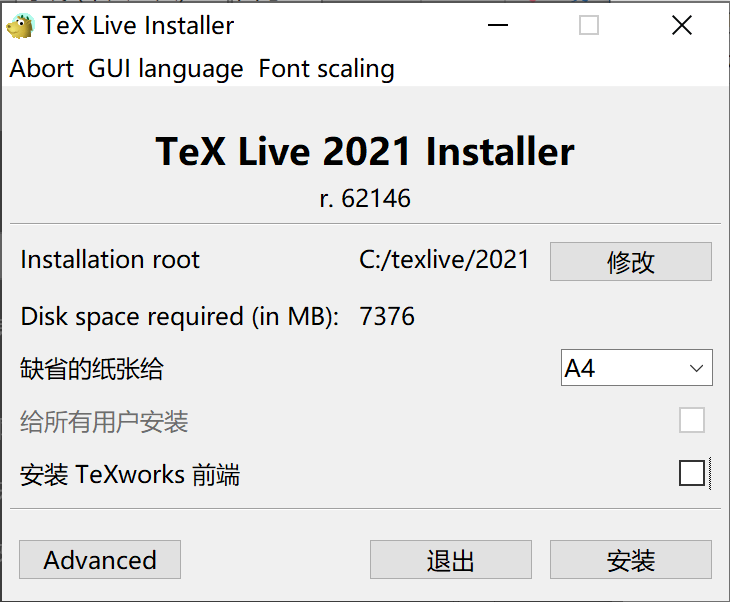
\includegraphics[width=0.45\textwidth]{install-tl-2}
  \caption{在线安装第二步。实际上跟本地安装是一样的,只不过版本较新。}
\end{figure}

全部完成后可以关闭安装程序,接着阅读 \ref{sec:hw}。

\subsection{macOS}
\label{subsec:tl-mac}

点击链接下载安装镜像:

\begin{itemize}
  \item \href{https://mirrors.nju.edu.cn/CTAN/systems/mac/mactex/mactex-20210328.pkg}{\faFile*[regular] Mac\hologo{TeX} 2021 安装镜像}
\end{itemize}

随后点击安装镜像,在安装程序中一路“继续”。

\begin{figure}[htbp]
  \caption{Mac\hologo{TeX} 2021 安装器。}
  \label{fig:install-mactex}
  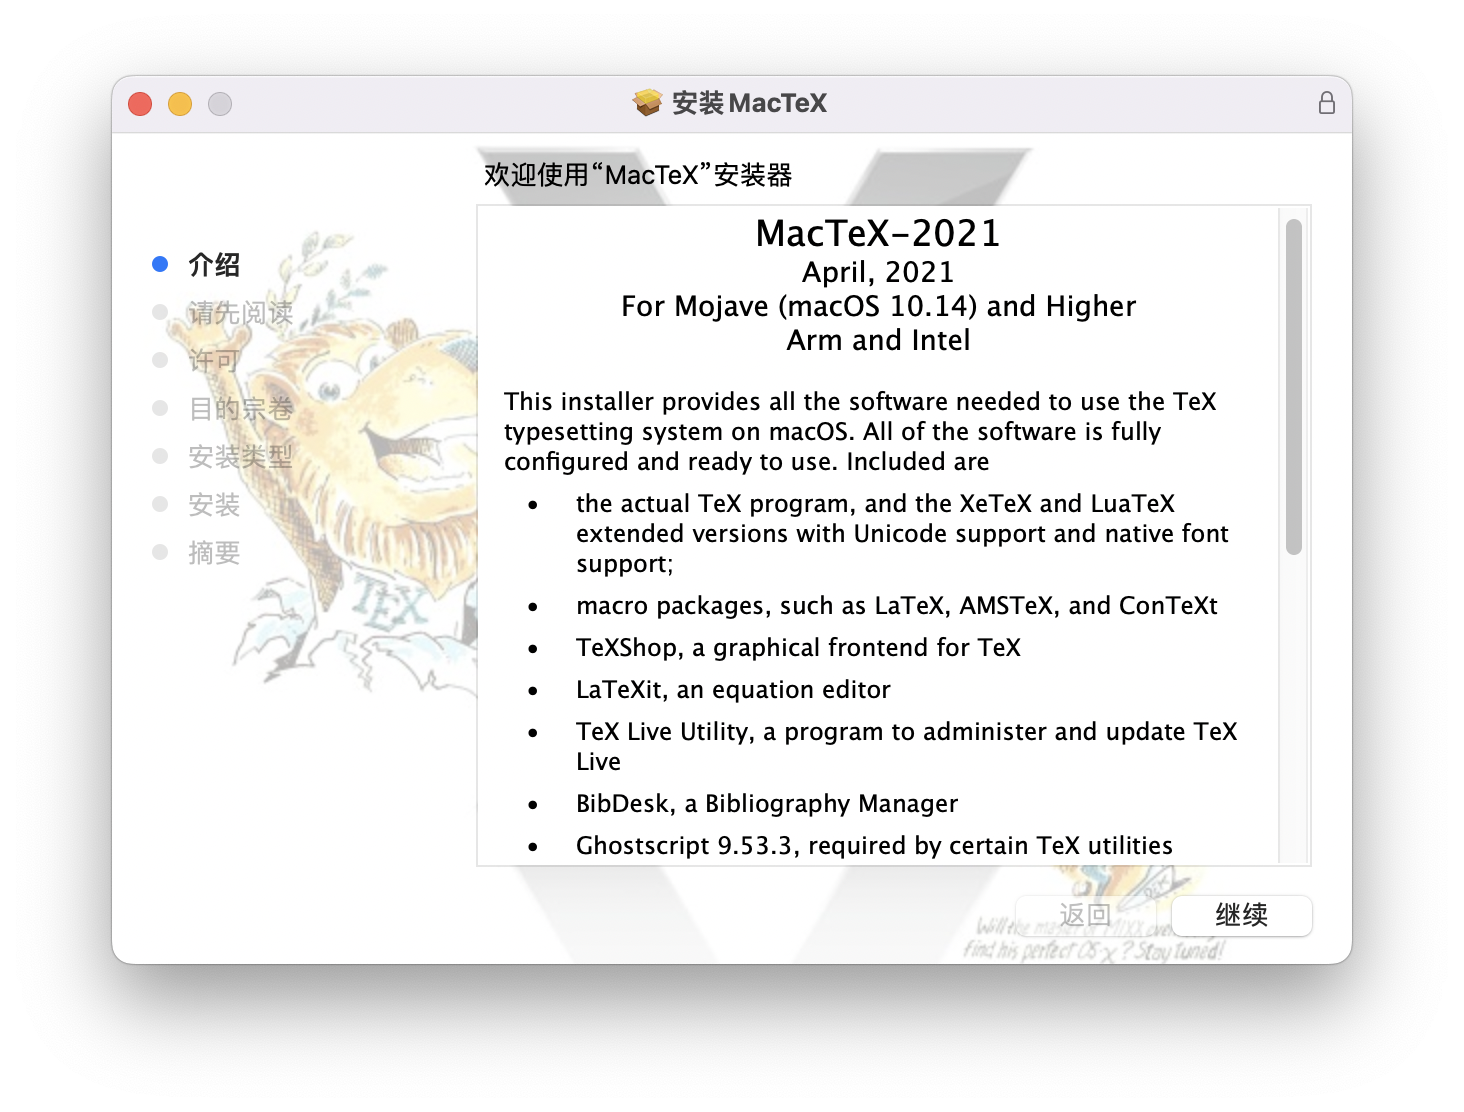
\includegraphics[width=0.75\textwidth]{install-mactex.png}
\end{figure}

静候安装完成,接着阅读 \ref{sec:hw}。

\subsection{Linux}
\label{subsec:tl-linux}

针对 Linux 系统,网络连接稳定时更推荐使用在线安装方式\sidenote{系统包管理器提供的版本往往较为落后}。首先下载安装器:

\begin{itemize}
  \item \href{https://mirrors.nju.edu.cn/CTAN/systems/texlive/tlnet/install-tl.zip}{\faFile*[regular] \texttt{install-tl.zip}}
\end{itemize}

\begin{widepar}
解压缩后,在 \texttt{install-tl} 文件所在的目录下打开终端,运行以下命令:

\begin{shellexample}[morekeywords={perl}]
  sudo perl install-tl --repository https://mirrors.nju.edu.cn/CTAN/systems/texlive/tlnet
\end{shellexample}

默认设置无需更改。键入 \texttt{i} 开始安装即可,预计用时约十分钟。

安装完成后,需要配置环境变量以使终端正确调用命令。以 Bash 为例,在 \texttt{~/.bashrc} 中添加以下内容:

\begin{textexample}
  PATH=/usr/local/texlive/2021/bin/x86_64-linux:$PATH; export PATH
  MANPATH=/usr/local/texlive/2021/texmf-dist/doc/man:$MANPATH; export MANPATH
  INFOPATH=/usr/local/texlive/2021/texmf-dist/doc/info:$INFOPATH; export INFOPATH
\end{textexample}

此外,为了使 tlmgr 能够以管理员身份执行,还需执行 \texttt{visudo},添加二进制文件所在目录。修改后形如:

\begin{textexample}
  Defaults secure_path="/usr/local/texlive/2021/bin/x86_64-linux:/usr/local/sbin:/usr/local/bin:/usr/sbin:/usr/bin:/sbin:/bin"
\end{textexample}

\end{widepar}
